\documentclass{standalone}
\usepackage{tikz}
\usetikzlibrary{patterns}
\usetikzlibrary{positioning}
\usetikzlibrary{patterns, positioning}
\usetikzlibrary{shapes.misc}
\usepackage[outline]{contour}
\contourlength{1.5pt} 
\usetikzlibrary{calc}
        \usepackage{relsize}
        \tikzset{fontscale/.style = {font=\relsize{#1}}}

\begin{document}
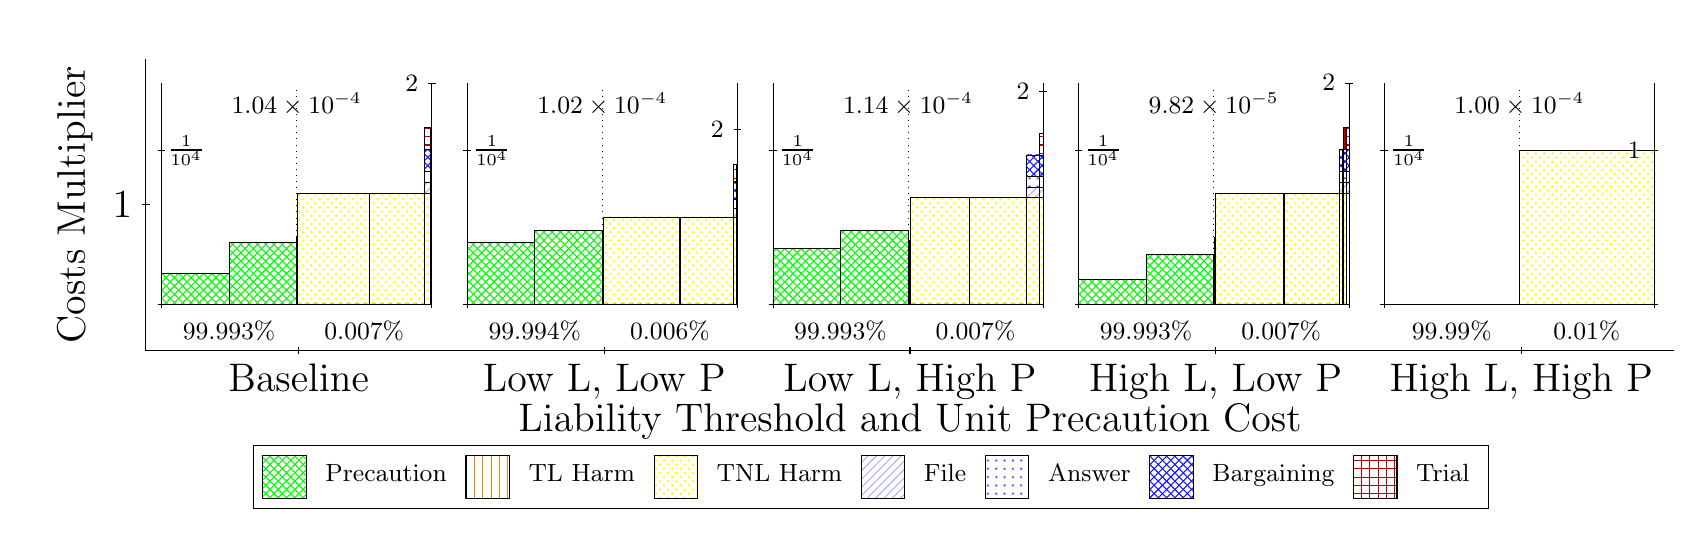
\begin{tikzpicture}
\clip(-0.5,-1.1) rectangle +(20.91,6.2);
\draw[black] (1,1) -- (1,4.7);
\node[rotate=90, fontscale=2, anchor=center] at (0.1, 2.85) {Costs Multiplier};
\draw[black] (0.95,2.85) -- (1.05,2.85);
\node[fontscale=2, anchor=east] at (0.95, 2.85) {1};

\draw[black] (1,1) -- (20.41,1);
\node[fontscale=2, anchor=center] at (10.705, 0.1) {Liability Threshold and Unit Precaution Cost};
\draw[black] (2.941,0.95) -- (2.941,1.05);
\node[fontscale=2, anchor=north] at (2.941, 0.95) {Baseline};
\draw[black] (6.823,0.95) -- (6.823,1.05);
\node[fontscale=2, anchor=north] at (6.823, 0.95) {Low L, Low P};
\draw[black] (10.705,0.95) -- (10.705,1.05);
\node[fontscale=2, anchor=north] at (10.705, 0.95) {Low L, High P};
\draw[black] (14.587,0.95) -- (14.587,1.05);
\node[fontscale=2, anchor=north] at (14.587, 0.95) {High L, Low P};
\draw[black] (18.469,0.95) -- (18.469,1.05);
\node[fontscale=2, anchor=north] at (18.469, 0.95) {High L, High P};


\draw[pattern=crosshatch, pattern color=green,draw=black,very thin] (1.2,1.592) rectangle (2.058,1.9821);
\draw[pattern=crosshatch, pattern color=green,draw=black,very thin] (2.058,1.592) rectangle (2.916,2.3722);
\draw[pattern=crosshatch, pattern color=green,draw=black,very thin] (2.916,1.592) rectangle (2.9275,1.592);
\draw[pattern=north east lines, pattern color=blue!30,draw=black,very thin] (2.916,1.592) rectangle (2.9275,1.7321);
\draw[pattern=dots,  pattern color=blue!60,draw=black,very thin] (2.916,1.7321) rectangle (2.9275,1.8722);
\draw[pattern=crosshatch,      pattern color=blue!90,draw=black,very thin] (2.916,1.8722) rectangle (2.9275,2.1524);
\draw[pattern=grid,            pattern color=red!70!black,draw=black,very thin] (2.916,2.1524) rectangle (2.9275,2.4326);
\draw[pattern=crosshatch, pattern color=green,draw=black,very thin] (2.9275,1.592) rectangle (3.8372,1.592);
\draw[pattern=crosshatch dots, pattern color=yellow,draw=black,very thin] (2.9275,1.592) rectangle (3.8372,2.993);
\draw[pattern=crosshatch, pattern color=green,draw=black,very thin] (3.8372,1.592) rectangle (3.8417,1.592);
\draw[pattern=vertical lines, pattern color=orange,draw=black,very thin] (3.8372,1.592) rectangle (3.8417,2.993);
\draw[pattern=crosshatch, pattern color=green,draw=black,very thin] (3.8417,1.592) rectangle (4.5413,1.5921);
\draw[pattern=crosshatch dots, pattern color=yellow,draw=black,very thin] (3.8417,1.5921) rectangle (4.5413,2.9931);
\draw[pattern=crosshatch, pattern color=green,draw=black,very thin] (4.5413,1.592) rectangle (4.6167,1.592);
\draw[pattern=crosshatch dots, pattern color=yellow,draw=black,very thin] (4.5413,1.592) rectangle (4.6167,2.993);
\draw[pattern=north east lines, pattern color=blue!30,draw=black,very thin] (4.5413,2.993) rectangle (4.6167,3.1331);
\draw[pattern=dots,  pattern color=blue!60,draw=black,very thin] (4.5413,3.1331) rectangle (4.6167,3.2732);
\draw[pattern=crosshatch,      pattern color=blue!90,draw=black,very thin] (4.5413,3.2732) rectangle (4.6167,3.5534);
\draw[pattern=grid,            pattern color=red!70!black,draw=black,very thin] (4.5413,3.5534) rectangle (4.6167,3.8336);
\draw[pattern=crosshatch, pattern color=green,draw=black,very thin] (4.6167,1.592) rectangle (4.632,1.592);
\draw[pattern=vertical lines, pattern color=orange,draw=black,very thin] (4.6167,1.592) rectangle (4.632,2.993);
\draw[pattern=north east lines, pattern color=blue!30,draw=black,very thin] (4.6167,2.993) rectangle (4.632,3.1331);
\draw[pattern=dots,  pattern color=blue!60,draw=black,very thin] (4.6167,3.1331) rectangle (4.632,3.2732);
\draw[pattern=crosshatch,      pattern color=blue!90,draw=black,very thin] (4.6167,3.2732) rectangle (4.632,3.5534);
\draw[pattern=grid,            pattern color=red!70!black,draw=black,very thin] (4.6167,3.5534) rectangle (4.632,3.8336);
\node[font=\small,text=black,anchor=north] at (2.916, 4.4) {$1.04\times 10^{-4}$};
\draw[black,very thin] (1.2,1.592) -- (1.2,4.4);
\draw[black,very thin] (1.15,1.592) -- (1.25,1.592);
\node[font=\small,text=black, anchor=west] at (1.15, 1.592) {};
\draw[black,very thin] (1.15,3.5425) -- (1.25,3.5425);
\node[font=\small,text=black, anchor=west] at (1.15, 3.5425) {$\frac{1}{10^{4}}$};

\draw[black,dotted,very thin] (2.916,1.6762) -- (2.916,4.3158);
\draw[black,very thin] (4.632,1.592) -- (4.632,4.4);
\draw[black,very thin] (4.582,4.394) -- (4.682,4.394);
\node[font=\small,text=black, anchor=east] at (4.582, 4.394) {\contour{white}{2}};

\draw[black,very thin] (1.2,1.592) -- (4.632,1.592);
\draw[black,very thin] (1.2,1.542) -- (1.2,1.642);
\node[font=\small,text=black, anchor=north] at (1.2, 1.542) {};
\draw[black,very thin] (4.632,1.542) -- (4.632,1.642);
\node[font=\small,text=black, anchor=north] at (4.632, 1.542) {};

\node[font=\small,text=black,anchor=south] at (2.058, 0.992) {99.993\%};
\node[font=\small,text=black,anchor=south] at (3.774, 0.992) {0.007\%};

\draw[pattern=crosshatch, pattern color=green,draw=black,very thin] (5.082,1.592) rectangle (5.94,2.3722);
\draw[pattern=crosshatch, pattern color=green,draw=black,very thin] (5.94,1.592) rectangle (6.798,2.5282);
\draw[pattern=crosshatch, pattern color=green,draw=black,very thin] (6.798,1.592) rectangle (6.8068,1.592);
\draw[pattern=north east lines, pattern color=blue!30,draw=black,very thin] (6.798,1.592) rectangle (6.8068,1.7027);
\draw[pattern=dots,  pattern color=blue!60,draw=black,very thin] (6.798,1.7027) rectangle (6.8068,1.8133);
\draw[pattern=crosshatch,      pattern color=blue!90,draw=black,very thin] (6.798,1.8133) rectangle (6.8068,2.0346);
\draw[pattern=grid,            pattern color=red!70!black,draw=black,very thin] (6.798,2.0346) rectangle (6.8068,2.2558);
\draw[pattern=crosshatch, pattern color=green,draw=black,very thin] (6.8068,1.592) rectangle (7.7764,1.592);
\draw[pattern=crosshatch dots, pattern color=yellow,draw=black,very thin] (6.8068,1.592) rectangle (7.7764,2.6983);
\draw[pattern=crosshatch, pattern color=green,draw=black,very thin] (7.7764,1.592) rectangle (7.7818,1.592);
\draw[pattern=vertical lines, pattern color=orange,draw=black,very thin] (7.7764,1.592) rectangle (7.7818,2.6983);
\draw[pattern=crosshatch, pattern color=green,draw=black,very thin] (7.7818,1.592) rectangle (8.4667,1.5921);
\draw[pattern=crosshatch dots, pattern color=yellow,draw=black,very thin] (7.7818,1.5921) rectangle (8.4667,2.6983);
\draw[pattern=crosshatch, pattern color=green,draw=black,very thin] (8.4667,1.592) rectangle (8.5039,1.592);
\draw[pattern=crosshatch dots, pattern color=yellow,draw=black,very thin] (8.4667,1.592) rectangle (8.5039,2.6983);
\draw[pattern=north east lines, pattern color=blue!30,draw=black,very thin] (8.4667,2.6983) rectangle (8.5039,2.809);
\draw[pattern=dots,  pattern color=blue!60,draw=black,very thin] (8.4667,2.809) rectangle (8.5039,2.9196);
\draw[pattern=crosshatch,      pattern color=blue!90,draw=black,very thin] (8.4667,2.9196) rectangle (8.5039,3.1408);
\draw[pattern=grid,            pattern color=red!70!black,draw=black,very thin] (8.4667,3.1408) rectangle (8.5039,3.3621);
\draw[pattern=crosshatch, pattern color=green,draw=black,very thin] (8.5039,1.592) rectangle (8.514,1.592);
\draw[pattern=vertical lines, pattern color=orange,draw=black,very thin] (8.5039,1.592) rectangle (8.514,2.6983);
\draw[pattern=north east lines, pattern color=blue!30,draw=black,very thin] (8.5039,2.6983) rectangle (8.514,2.809);
\draw[pattern=dots,  pattern color=blue!60,draw=black,very thin] (8.5039,2.809) rectangle (8.514,2.9196);
\draw[pattern=crosshatch,      pattern color=blue!90,draw=black,very thin] (8.5039,2.9196) rectangle (8.514,3.1408);
\draw[pattern=grid,            pattern color=red!70!black,draw=black,very thin] (8.5039,3.1408) rectangle (8.514,3.3621);
\node[font=\small,text=black,anchor=north] at (6.798, 4.4) {$1.02\times 10^{-4}$};
\draw[black,very thin] (5.082,1.592) -- (5.082,4.4);
\draw[black,very thin] (5.032,1.592) -- (5.132,1.592);
\node[font=\small,text=black, anchor=west] at (5.032, 1.592) {};
\draw[black,very thin] (5.032,3.5425) -- (5.132,3.5425);
\node[font=\small,text=black, anchor=west] at (5.032, 3.5425) {$\frac{1}{10^{4}}$};

\draw[black,dotted,very thin] (6.798,1.6762) -- (6.798,4.3158);
\draw[black,very thin] (8.514,1.592) -- (8.514,4.4);
\draw[black,very thin] (8.464,3.8046) -- (8.564,3.8046);
\node[font=\small,text=black, anchor=east] at (8.464, 3.8046) {\contour{white}{2}};

\draw[black,very thin] (5.082,1.592) -- (8.514,1.592);
\draw[black,very thin] (5.082,1.542) -- (5.082,1.642);
\node[font=\small,text=black, anchor=north] at (5.082, 1.542) {};
\draw[black,very thin] (8.514,1.542) -- (8.514,1.642);
\node[font=\small,text=black, anchor=north] at (8.514, 1.542) {};

\node[font=\small,text=black,anchor=south] at (5.94, 0.992) {99.994\%};
\node[font=\small,text=black,anchor=south] at (7.656, 0.992) {0.006\%};

\draw[pattern=crosshatch, pattern color=green,draw=black,very thin] (8.964,1.592) rectangle (9.822,2.2942);
\draw[pattern=crosshatch, pattern color=green,draw=black,very thin] (9.822,1.592) rectangle (10.68,2.5282);
\draw[pattern=crosshatch, pattern color=green,draw=black,very thin] (10.68,1.592) rectangle (10.702,1.592);
\draw[pattern=north east lines, pattern color=blue!30,draw=black,very thin] (10.68,1.592) rectangle (10.702,1.7272);
\draw[pattern=dots,  pattern color=blue!60,draw=black,very thin] (10.68,1.7272) rectangle (10.702,1.8623);
\draw[pattern=crosshatch,      pattern color=blue!90,draw=black,very thin] (10.68,1.8623) rectangle (10.702,2.1325);
\draw[pattern=crosshatch, pattern color=green,draw=black,very thin] (10.702,1.592) rectangle (10.709,1.592);
\draw[pattern=north east lines, pattern color=blue!30,draw=black,very thin] (10.702,1.592) rectangle (10.709,1.7272);
\draw[pattern=dots,  pattern color=blue!60,draw=black,very thin] (10.702,1.7272) rectangle (10.709,1.8623);
\draw[pattern=crosshatch,      pattern color=blue!90,draw=black,very thin] (10.702,1.8623) rectangle (10.709,2.1325);
\draw[pattern=grid,            pattern color=red!70!black,draw=black,very thin] (10.702,2.1325) rectangle (10.709,2.4028);
\draw[pattern=crosshatch, pattern color=green,draw=black,very thin] (10.709,1.592) rectangle (11.458,1.592);
\draw[pattern=crosshatch dots, pattern color=yellow,draw=black,very thin] (10.709,1.592) rectangle (11.458,2.9433);
\draw[pattern=crosshatch, pattern color=green,draw=black,very thin] (11.458,1.592) rectangle (12.183,1.5921);
\draw[pattern=crosshatch dots, pattern color=yellow,draw=black,very thin] (11.458,1.5921) rectangle (12.183,2.9433);
\draw[pattern=crosshatch, pattern color=green,draw=black,very thin] (12.183,1.592) rectangle (12.346,1.592);
\draw[pattern=crosshatch dots, pattern color=yellow,draw=black,very thin] (12.183,1.592) rectangle (12.346,2.9433);
\draw[pattern=north east lines, pattern color=blue!30,draw=black,very thin] (12.183,2.9433) rectangle (12.346,3.0784);
\draw[pattern=dots,  pattern color=blue!60,draw=black,very thin] (12.183,3.0784) rectangle (12.346,3.2135);
\draw[pattern=crosshatch,      pattern color=blue!90,draw=black,very thin] (12.183,3.2135) rectangle (12.346,3.4838);
\draw[pattern=crosshatch, pattern color=green,draw=black,very thin] (12.346,1.592) rectangle (12.347,1.592);
\draw[pattern=vertical lines, pattern color=orange,draw=black,very thin] (12.346,1.592) rectangle (12.347,2.9433);
\draw[pattern=north east lines, pattern color=blue!30,draw=black,very thin] (12.346,2.9433) rectangle (12.347,3.0784);
\draw[pattern=dots,  pattern color=blue!60,draw=black,very thin] (12.346,3.0784) rectangle (12.347,3.2135);
\draw[pattern=crosshatch,      pattern color=blue!90,draw=black,very thin] (12.346,3.2135) rectangle (12.347,3.4838);
\draw[pattern=crosshatch, pattern color=green,draw=black,very thin] (12.347,1.592) rectangle (12.393,1.592);
\draw[pattern=crosshatch dots, pattern color=yellow,draw=black,very thin] (12.347,1.592) rectangle (12.393,2.9433);
\draw[pattern=north east lines, pattern color=blue!30,draw=black,very thin] (12.347,2.9433) rectangle (12.393,3.0784);
\draw[pattern=dots,  pattern color=blue!60,draw=black,very thin] (12.347,3.0784) rectangle (12.393,3.2135);
\draw[pattern=crosshatch,      pattern color=blue!90,draw=black,very thin] (12.347,3.2135) rectangle (12.393,3.4838);
\draw[pattern=grid,            pattern color=red!70!black,draw=black,very thin] (12.347,3.4838) rectangle (12.393,3.754);
\draw[pattern=crosshatch, pattern color=green,draw=black,very thin] (12.393,1.592) rectangle (12.396,1.592);
\draw[pattern=vertical lines, pattern color=orange,draw=black,very thin] (12.393,1.592) rectangle (12.396,2.9433);
\draw[pattern=north east lines, pattern color=blue!30,draw=black,very thin] (12.393,2.9433) rectangle (12.396,3.0784);
\draw[pattern=dots,  pattern color=blue!60,draw=black,very thin] (12.393,3.0784) rectangle (12.396,3.2135);
\draw[pattern=crosshatch,      pattern color=blue!90,draw=black,very thin] (12.393,3.2135) rectangle (12.396,3.4838);
\draw[pattern=grid,            pattern color=red!70!black,draw=black,very thin] (12.393,3.4838) rectangle (12.396,3.754);
\node[font=\small,text=black,anchor=north] at (10.68, 4.4) {$1.14\times 10^{-4}$};
\draw[black,very thin] (8.964,1.592) -- (8.964,4.4);
\draw[black,very thin] (8.914,1.592) -- (9.014,1.592);
\node[font=\small,text=black, anchor=west] at (8.914, 1.592) {};
\draw[black,very thin] (8.914,3.5425) -- (9.014,3.5425);
\node[font=\small,text=black, anchor=west] at (8.914, 3.5425) {$\frac{1}{10^{4}}$};

\draw[black,dotted,very thin] (10.68,1.6762) -- (10.68,4.3158);
\draw[black,very thin] (12.396,1.592) -- (12.396,4.4);
\draw[black,very thin] (12.346,4.2945) -- (12.446,4.2945);
\node[font=\small,text=black, anchor=east] at (12.346, 4.2945) {\contour{white}{2}};

\draw[black,very thin] (8.964,1.592) -- (12.396,1.592);
\draw[black,very thin] (8.964,1.542) -- (8.964,1.642);
\node[font=\small,text=black, anchor=north] at (8.964, 1.542) {};
\draw[black,very thin] (12.396,1.542) -- (12.396,1.642);
\node[font=\small,text=black, anchor=north] at (12.396, 1.542) {};

\node[font=\small,text=black,anchor=south] at (9.822, 0.992) {99.993\%};
\node[font=\small,text=black,anchor=south] at (11.538, 0.992) {0.007\%};

\draw[pattern=crosshatch, pattern color=green,draw=black,very thin] (12.846,1.592) rectangle (13.704,1.9041);
\draw[pattern=crosshatch, pattern color=green,draw=black,very thin] (13.704,1.592) rectangle (14.562,2.2162);
\draw[pattern=crosshatch, pattern color=green,draw=black,very thin] (14.562,1.592) rectangle (14.569,1.592);
\draw[pattern=north east lines, pattern color=blue!30,draw=black,very thin] (14.562,1.592) rectangle (14.569,1.7324);
\draw[pattern=dots,  pattern color=blue!60,draw=black,very thin] (14.562,1.7324) rectangle (14.569,1.8728);
\draw[pattern=crosshatch,      pattern color=blue!90,draw=black,very thin] (14.562,1.8728) rectangle (14.569,2.1536);
\draw[pattern=crosshatch, pattern color=green,draw=black,very thin] (14.569,1.592) rectangle (14.577,1.592);
\draw[pattern=north east lines, pattern color=blue!30,draw=black,very thin] (14.569,1.592) rectangle (14.577,1.7324);
\draw[pattern=dots,  pattern color=blue!60,draw=black,very thin] (14.569,1.7324) rectangle (14.577,1.8728);
\draw[pattern=crosshatch,      pattern color=blue!90,draw=black,very thin] (14.569,1.8728) rectangle (14.577,2.1536);
\draw[pattern=grid,            pattern color=red!70!black,draw=black,very thin] (14.569,2.1536) rectangle (14.577,2.4344);
\draw[pattern=crosshatch, pattern color=green,draw=black,very thin] (14.577,1.592) rectangle (15.444,1.592);
\draw[pattern=crosshatch dots, pattern color=yellow,draw=black,very thin] (14.577,1.592) rectangle (15.444,2.996);
\draw[pattern=crosshatch, pattern color=green,draw=black,very thin] (15.444,1.592) rectangle (15.46,1.592);
\draw[pattern=vertical lines, pattern color=orange,draw=black,very thin] (15.444,1.592) rectangle (15.46,2.996);
\draw[pattern=crosshatch, pattern color=green,draw=black,very thin] (15.46,1.592) rectangle (16.158,1.592);
\draw[pattern=crosshatch dots, pattern color=yellow,draw=black,very thin] (15.46,1.592) rectangle (16.158,2.996);
\draw[pattern=crosshatch, pattern color=green,draw=black,very thin] (16.158,1.592) rectangle (16.2,1.592);
\draw[pattern=crosshatch dots, pattern color=yellow,draw=black,very thin] (16.158,1.592) rectangle (16.2,2.996);
\draw[pattern=north east lines, pattern color=blue!30,draw=black,very thin] (16.158,2.996) rectangle (16.2,3.1364);
\draw[pattern=dots,  pattern color=blue!60,draw=black,very thin] (16.158,3.1364) rectangle (16.2,3.2768);
\draw[pattern=crosshatch,      pattern color=blue!90,draw=black,very thin] (16.158,3.2768) rectangle (16.2,3.5576);
\draw[pattern=crosshatch, pattern color=green,draw=black,very thin] (16.2,1.592) rectangle (16.213,1.592);
\draw[pattern=vertical lines, pattern color=orange,draw=black,very thin] (16.2,1.592) rectangle (16.213,2.996);
\draw[pattern=north east lines, pattern color=blue!30,draw=black,very thin] (16.2,2.996) rectangle (16.213,3.1364);
\draw[pattern=dots,  pattern color=blue!60,draw=black,very thin] (16.2,3.1364) rectangle (16.213,3.2768);
\draw[pattern=crosshatch,      pattern color=blue!90,draw=black,very thin] (16.2,3.2768) rectangle (16.213,3.5576);
\draw[pattern=crosshatch, pattern color=green,draw=black,very thin] (16.213,1.592) rectangle (16.247,1.592);
\draw[pattern=crosshatch dots, pattern color=yellow,draw=black,very thin] (16.213,1.592) rectangle (16.247,2.996);
\draw[pattern=north east lines, pattern color=blue!30,draw=black,very thin] (16.213,2.996) rectangle (16.247,3.1364);
\draw[pattern=dots,  pattern color=blue!60,draw=black,very thin] (16.213,3.1364) rectangle (16.247,3.2768);
\draw[pattern=crosshatch,      pattern color=blue!90,draw=black,very thin] (16.213,3.2768) rectangle (16.247,3.5576);
\draw[pattern=grid,            pattern color=red!70!black,draw=black,very thin] (16.213,3.5576) rectangle (16.247,3.8384);
\draw[pattern=crosshatch, pattern color=green,draw=black,very thin] (16.247,1.592) rectangle (16.278,1.592);
\draw[pattern=vertical lines, pattern color=orange,draw=black,very thin] (16.247,1.592) rectangle (16.278,2.996);
\draw[pattern=north east lines, pattern color=blue!30,draw=black,very thin] (16.247,2.996) rectangle (16.278,3.1364);
\draw[pattern=dots,  pattern color=blue!60,draw=black,very thin] (16.247,3.1364) rectangle (16.278,3.2768);
\draw[pattern=crosshatch,      pattern color=blue!90,draw=black,very thin] (16.247,3.2768) rectangle (16.278,3.5576);
\draw[pattern=grid,            pattern color=red!70!black,draw=black,very thin] (16.247,3.5576) rectangle (16.278,3.8384);
\node[font=\small,text=black,anchor=north] at (14.562, 4.4) {$9.82\times 10^{-5}$};
\draw[black,very thin] (12.846,1.592) -- (12.846,4.4);
\draw[black,very thin] (12.796,1.592) -- (12.896,1.592);
\node[font=\small,text=black, anchor=west] at (12.796, 1.592) {};
\draw[black,very thin] (12.796,3.5425) -- (12.896,3.5425);
\node[font=\small,text=black, anchor=west] at (12.796, 3.5425) {$\frac{1}{10^{4}}$};

\draw[black,dotted,very thin] (14.562,1.6762) -- (14.562,4.3158);
\draw[black,very thin] (16.278,1.592) -- (16.278,4.4);
\draw[black,very thin] (16.228,4.4) -- (16.328,4.4);
\node[font=\small,text=black, anchor=east] at (16.228, 4.4) {\contour{white}{2}};

\draw[black,very thin] (12.846,1.592) -- (16.278,1.592);
\draw[black,very thin] (12.846,1.542) -- (12.846,1.642);
\node[font=\small,text=black, anchor=north] at (12.846, 1.542) {};
\draw[black,very thin] (16.278,1.542) -- (16.278,1.642);
\node[font=\small,text=black, anchor=north] at (16.278, 1.542) {};

\node[font=\small,text=black,anchor=south] at (13.704, 0.992) {99.993\%};
\node[font=\small,text=black,anchor=south] at (15.42, 0.992) {0.007\%};

\draw[pattern=crosshatch dots, pattern color=yellow,draw=black,very thin] (18.444,1.592) rectangle (20.16,3.5426);
\node[font=\small,text=black,anchor=north] at (18.444, 4.4) {$1.00\times 10^{-4}$};
\draw[black,very thin] (16.728,1.592) -- (16.728,4.4);
\draw[black,very thin] (16.678,1.592) -- (16.778,1.592);
\node[font=\small,text=black, anchor=west] at (16.678, 1.592) {};
\draw[black,very thin] (16.678,3.5424) -- (16.778,3.5424);
\node[font=\small,text=black, anchor=west] at (16.678, 3.5424) {$\frac{1}{10^{4}}$};

\draw[black,dotted,very thin] (18.444,1.6762) -- (18.444,4.3158);
\draw[black,very thin] (20.16,1.592) -- (20.16,4.4);
\draw[black,very thin] (20.11,1.592) -- (20.21,1.592);
\node[font=\small,text=black, anchor=east] at (20.11, 1.592) {\contour{white}{}};
\draw[black,very thin] (20.11,3.5426) -- (20.21,3.5426);
\node[font=\small,text=black, anchor=east] at (20.11, 3.5426) {\contour{white}{1}};

\draw[black,very thin] (16.728,1.592) -- (20.16,1.592);
\draw[black,very thin] (16.728,1.542) -- (16.728,1.642);
\node[font=\small,text=black, anchor=north] at (16.728, 1.542) {};
\draw[black,very thin] (20.16,1.542) -- (20.16,1.642);
\node[font=\small,text=black, anchor=north] at (20.16, 1.542) {};

\node[font=\small,text=black,anchor=south] at (17.586, 0.992) {99.99\%};
\node[font=\small,text=black,anchor=south] at (19.302, 0.992) {0.01\%};

\coordinate (LegendAnchor) at (10.205000000000002,0);
\begin{scope}[align=center]
\matrix[scale=0.6,draw=black,below=0.2cm of LegendAnchor,nodes={draw},column sep=0.12cm]{
\node[rectangle,draw,minimum width=0.55cm,minimum height=0.55cm,pattern=crosshatch, pattern color=green]{}; &
        \node[draw=none,font=\small]{Precaution}; &
\node[rectangle,draw,minimum width=0.55cm,minimum height=0.55cm,pattern=vertical lines, pattern color=orange]{}; &
        \node[draw=none,font=\small]{TL Harm}; &
\node[rectangle,draw,minimum width=0.55cm,minimum height=0.55cm,pattern=crosshatch dots, pattern color=yellow]{}; &
        \node[draw=none,font=\small]{TNL Harm}; &
\node[rectangle,draw,minimum width=0.55cm,minimum height=0.55cm,pattern=north east lines, pattern color=blue!30]{}; &
        \node[draw=none,font=\small]{File}; &
\node[rectangle,draw,minimum width=0.55cm,minimum height=0.55cm,pattern=dots, pattern color=blue!60]{}; &
        \node[draw=none,font=\small]{Answer}; &
\node[rectangle,draw,minimum width=0.55cm,minimum height=0.55cm,pattern=crosshatch, pattern color=blue!90]{}; &
        \node[draw=none,font=\small]{Bargaining}; &
\node[rectangle,draw,minimum width=0.55cm,minimum height=0.55cm,pattern=grid, pattern color=red!70!black]{}; &
        \node[draw=none,font=\small]{Trial}; \\
};\end{scope}

\end{tikzpicture}
\end{document}